\documentclass[usenames,dvipsnames,tikz]{standalone}
\usetikzlibrary{patterns}
%\usetikzlibrary{shapes.geometric}
%\usepackage{xcolor}
\colorlet{tBlue}{RoyalBlue!35!Cerulean}
\colorlet{tRed}{Red}
%\definecolor{tGreen}{HTML}{569909}
%\definecolor{tOrange}{HTML}{FA7602}
\usepackage{tikz}
\usepackage{standalone}
\begin{document}	
	
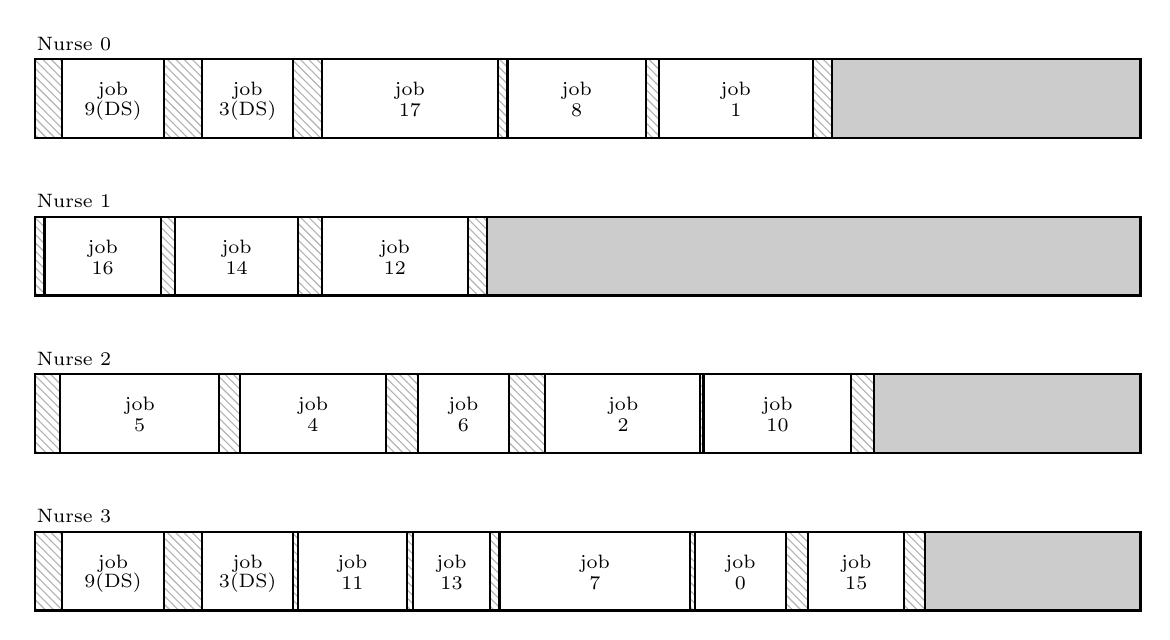
\begin{tikzpicture}
%\draw [help lines] (-1,-1) grid (15,8);

% Nurse 0
\draw [thick] (0,6) rectangle (14.04, 7);
\draw [thick, pattern = north west lines, pattern color=black!30!white] (0,6) rectangle (0.34,7);
\draw [thick] (0.34,6) -- (0.34,7); % start of job 9
\draw [thick] (1.64,6) -- (1.64,7); % end of job 9
\draw [thick, pattern = north west lines, pattern color=black!30!white] (1.64,6) rectangle (2.12,7);
\draw [thick] (2.12,6) -- (2.12,7); % start of job 3
\draw [thick] (3.28,6) -- (3.28,7); % end of job 3
\draw [thick, pattern = north west lines, pattern color=black!30!white] (3.28,6) rectangle (3.64,7);
\draw [thick] (3.64,6) -- (3.64,7); % start of job 17
\draw [thick] (5.88,6) -- (5.88,7); % end of job 17
\draw [thick, pattern = north west lines, pattern color=black!30!white] (5.88,6) rectangle (6.00,7);
\draw [thick] (6.00,6) -- (6.00,7); % start of job 8
\draw [thick] (7.76,6) -- (7.76,7); % end of job 8
\draw [thick, pattern = north west lines, pattern color=black!30!white] (7.76,6) rectangle (7.92,7);
\draw [thick] (7.92,6) -- (7.92,7); % start of job 1
\draw [thick] (9.88,6) -- (9.88,7); % end of job 1
\draw [thick, pattern = north west lines, pattern color=black!30!white] (9.88,6) rectangle (10.12,7);
\draw [thick] (10.12,6) -- (10.12,7); % end of shift
\draw [thick, fill=black!20!white] (10.12,6) rectangle (14.04,7);

\node [right] at (-0.1,7.2) {\scriptsize{Nurse 0}};
\node at (0.99,6.6) {\scriptsize{job}}; 
\node at (0.99,6.35) {\scriptsize{9(DS)}};
\node at (2.70,6.6) {\scriptsize{job}};
\node at (2.70,6.35) {\scriptsize{3(DS)}};
\node at (4.76,6.6) {\scriptsize{job}};
\node at (4.76,6.35) {\scriptsize{17}};
\node at (6.88,6.6) {\scriptsize{job}};
\node at (6.88,6.35) {\scriptsize{8}};
\node at (8.90,6.6) {\scriptsize{job}};
\node at (8.90,6.35) {\scriptsize{1}};



% Nurse 1
\draw [thick] (0,4) rectangle (14.04, 5);
\draw [thick, pattern = north west lines, pattern color=black!30!white] (0,4) rectangle (0.12,5);
\draw [thick] (0.12,4) -- (0.12,5); % start of job 16
\draw [thick] (1.60,4) -- (1.60,5); % end of job 16
\draw [thick, pattern = north west lines, pattern color=black!30!white] (1.60,4) rectangle (1.78,5);
\draw [thick] (1.78,4) -- (1.78,5); % start of job 14
\draw [thick] (3.34,4) -- (3.34,5); % end of job 14
\draw [thick, pattern = north west lines, pattern color=black!30!white] (3.34,4) rectangle (3.64,5);
\draw [thick] (3.64,4) -- (3.64,5); % start of job 12
\draw [thick] (5.50,4) -- (5.50,5); % end of job 12
\draw [thick, pattern = north west lines, pattern color=black!30!white] (5.50,4) rectangle (5.74,5);
\draw [thick] (5.74,4) -- (5.74,5); % end of shift
\draw [thick, fill=black!20!white] (5.74,4) rectangle (14.04,5);

\node [right] at (-0.1,5.2) {\scriptsize{Nurse 1}};
\node at (0.86,4.6) {\scriptsize{job}}; 
\node at (0.86,4.35) {\scriptsize{16}};
\node at (2.56,4.6) {\scriptsize{job}}; 
\node at (2.56,4.35) {\scriptsize{14}};
\node at (4.57,4.6) {\scriptsize{job}}; 
\node at (4.57,4.35) {\scriptsize{12}};


% Nurse 2
\draw [thick] (0,2) rectangle (14.04, 3);
\draw [thick, pattern = north west lines, pattern color=black!30!white] (0,2) rectangle (0.32,3);
\draw [thick] (0.32,2) -- (0.32,3); % start of job 5
\draw [thick] (2.34,2) -- (2.34,3); % end of job 5
\draw [thick, pattern = north west lines, pattern color=black!30!white] (2.34,2) rectangle (2.60,3);
\draw [thick] (2.60,2) -- (2.60,3); % start of job 4
\draw [thick] (4.46,2) -- (4.46,3); % end of job 4
\draw [thick, pattern = north west lines, pattern color=black!30!white] (4.46,2) rectangle (4.86,3);
\draw [thick] (4.86,2) -- (4.86,3); % start of job 6
\draw [thick] (6.02,2) -- (6.02,3); % end of job 6
\draw [thick, pattern = north west lines, pattern color=black!30!white] (6.02,2) rectangle (6.48,3);
\draw [thick] (6.48,2) -- (6.48,3); % start of job 2
\draw [thick] (8.45,2) -- (8.45,3); % end of job 2
\draw [thick, pattern = north west lines, pattern color=black!30!white] (8.45,2) rectangle (8.49,3);
\draw [thick] (8.49,2) -- (8.49,3); % start of job 10
\draw [thick] (10.36,2) -- (10.36,3); % end of job 10
\draw [thick, pattern = north west lines, pattern color=black!30!white] (10.36,2) rectangle (10.66,3);
\draw [thick] (10.66,2) -- (10.66,3); % end of shift
\draw [thick,fill=black!20!white] (10.66,2) rectangle (14.04,3);

\node [right] at (-0.1,3.2) {\scriptsize{Nurse 2}};
\node at (1.33,2.6) {\scriptsize{job}}; 
\node at (1.33,2.35) {\scriptsize{5}};
\node at (3.53,2.6) {\scriptsize{job}}; 
\node at (3.53,2.35) {\scriptsize{4}};
\node at (5.44,2.6) {\scriptsize{job}}; 
\node at (5.44,2.35) {\scriptsize{6}};
\node at (7.47,2.6) {\scriptsize{job}}; 
\node at (7.47,2.35) {\scriptsize{2}};
\node at (9.43,2.6) {\scriptsize{job}}; 
\node at (9.43,2.35) {\scriptsize{10}};


% Nurse 3
\draw [thick] (0,0) rectangle (14.04, 1);
\draw [thick, pattern = north west lines, pattern color=black!30!white] (0,0) rectangle (0.34,1);
\draw [thick] (0.34,0) -- (0.34,1); % start of job 9
\draw [thick] (1.64,0) -- (1.64,1); % end of job 9
\draw [thick, pattern = north west lines, pattern color=black!30!white] (1.64,0) rectangle (2.12,1);
\draw [thick] (2.12,0) -- (2.12,1); % start of job 3
\draw [thick] (3.28,0) -- (3.28,1); % end of job 3
\draw [thick, pattern = north west lines, pattern color=black!30!white] (3.28,0) rectangle (3.34,1);
\draw [thick] (3.34,0) -- (3.34,1); % start of job 11
\draw [thick] (4.72,0) -- (4.72,1); % end of job 11
\draw [thick, pattern = north west lines, pattern color=black!30!white] (4.72,0) rectangle (4.80,1);
\draw [thick] (4.80,0) -- (4.80,1); % start of job 13
\draw [thick] (5.78,0) -- (5.78,1); % end of job 13
\draw [thick, pattern = north west lines, pattern color=black!30!white] (5.78,0) rectangle (5.90,1);
\draw [thick] (5.90,0) -- (5.90,1); % start of job 7
\draw [thick] (8.32,0) -- (8.32,1); % end of job 7
\draw [thick, pattern = north west lines, pattern color=black!30!white] (8.32,0) rectangle (8.38,1);
\draw [thick] (8.38,0) -- (8.38,1); % start of job 0
\draw [thick] (9.54,0) -- (9.54,1); % end of job 0
\draw [thick, pattern = north west lines, pattern color=black!30!white] (9.54,0) rectangle (9.82,1);
\draw [thick] (9.82,0) -- (9.82,1); % start of job 15
\draw [thick] (11.04,0) -- (11.04,1); % end of job 15
\draw [thick, pattern = north west lines, pattern color=black!30!white] (11.04,0) rectangle (11.30,1);
\draw [thick] (11.30,0) -- (11.30,1); % end of shift
\draw [thick, fill=black!20!white] (11.30,0) rectangle (14.04,1);

\node [right] at (-0.1,1.2) {\scriptsize{Nurse 3}};
\node at (0.99,0.6) {\scriptsize{job}}; 
\node at (0.99,0.35) {\scriptsize{9(DS)}};
\node at (2.70,0.6) {\scriptsize{job}}; 
\node at (2.70,0.35) {\scriptsize{3(DS)}};
\node at (4.03,0.6) {\scriptsize{job}}; 
\node at (4.03,0.35) {\scriptsize{11}};
\node at (5.29,0.6) {\scriptsize{job}}; 
\node at (5.29,0.35) {\scriptsize{13}};
\node at (7.11,0.6) {\scriptsize{job}}; 
\node at (7.11,0.35) {\scriptsize{7}};
\node at (8.96,0.6) {\scriptsize{job}}; 
\node at (8.96,0.35) {\scriptsize{0}};
\node at (10.43,0.6) {\scriptsize{job}}; 
\node at (10.43,0.35) {\scriptsize{15}};






\end{tikzpicture}
	
\end{document}



